\documentclass[]{book}
\usepackage{lmodern}
\usepackage{amssymb,amsmath}
\usepackage{ifxetex,ifluatex}
\usepackage{fixltx2e} % provides \textsubscript
\ifnum 0\ifxetex 1\fi\ifluatex 1\fi=0 % if pdftex
  \usepackage[T1]{fontenc}
  \usepackage[utf8]{inputenc}
\else % if luatex or xelatex
  \ifxetex
    \usepackage{mathspec}
  \else
    \usepackage{fontspec}
  \fi
  \defaultfontfeatures{Ligatures=TeX,Scale=MatchLowercase}
\fi
% use upquote if available, for straight quotes in verbatim environments
\IfFileExists{upquote.sty}{\usepackage{upquote}}{}
% use microtype if available
\IfFileExists{microtype.sty}{%
\usepackage{microtype}
\UseMicrotypeSet[protrusion]{basicmath} % disable protrusion for tt fonts
}{}
\usepackage[margin=1in]{geometry}
\usepackage{hyperref}
\hypersetup{unicode=true,
            pdftitle={Similitud de Comunidades biológicas},
            pdfauthor={Carlos Iván Espinosa},
            pdfborder={0 0 0},
            breaklinks=true}
\urlstyle{same}  % don't use monospace font for urls
\usepackage{natbib}
\bibliographystyle{apalike}
\usepackage{color}
\usepackage{fancyvrb}
\newcommand{\VerbBar}{|}
\newcommand{\VERB}{\Verb[commandchars=\\\{\}]}
\DefineVerbatimEnvironment{Highlighting}{Verbatim}{commandchars=\\\{\}}
% Add ',fontsize=\small' for more characters per line
\usepackage{framed}
\definecolor{shadecolor}{RGB}{248,248,248}
\newenvironment{Shaded}{\begin{snugshade}}{\end{snugshade}}
\newcommand{\KeywordTok}[1]{\textcolor[rgb]{0.13,0.29,0.53}{\textbf{{#1}}}}
\newcommand{\DataTypeTok}[1]{\textcolor[rgb]{0.13,0.29,0.53}{{#1}}}
\newcommand{\DecValTok}[1]{\textcolor[rgb]{0.00,0.00,0.81}{{#1}}}
\newcommand{\BaseNTok}[1]{\textcolor[rgb]{0.00,0.00,0.81}{{#1}}}
\newcommand{\FloatTok}[1]{\textcolor[rgb]{0.00,0.00,0.81}{{#1}}}
\newcommand{\ConstantTok}[1]{\textcolor[rgb]{0.00,0.00,0.00}{{#1}}}
\newcommand{\CharTok}[1]{\textcolor[rgb]{0.31,0.60,0.02}{{#1}}}
\newcommand{\SpecialCharTok}[1]{\textcolor[rgb]{0.00,0.00,0.00}{{#1}}}
\newcommand{\StringTok}[1]{\textcolor[rgb]{0.31,0.60,0.02}{{#1}}}
\newcommand{\VerbatimStringTok}[1]{\textcolor[rgb]{0.31,0.60,0.02}{{#1}}}
\newcommand{\SpecialStringTok}[1]{\textcolor[rgb]{0.31,0.60,0.02}{{#1}}}
\newcommand{\ImportTok}[1]{{#1}}
\newcommand{\CommentTok}[1]{\textcolor[rgb]{0.56,0.35,0.01}{\textit{{#1}}}}
\newcommand{\DocumentationTok}[1]{\textcolor[rgb]{0.56,0.35,0.01}{\textbf{\textit{{#1}}}}}
\newcommand{\AnnotationTok}[1]{\textcolor[rgb]{0.56,0.35,0.01}{\textbf{\textit{{#1}}}}}
\newcommand{\CommentVarTok}[1]{\textcolor[rgb]{0.56,0.35,0.01}{\textbf{\textit{{#1}}}}}
\newcommand{\OtherTok}[1]{\textcolor[rgb]{0.56,0.35,0.01}{{#1}}}
\newcommand{\FunctionTok}[1]{\textcolor[rgb]{0.00,0.00,0.00}{{#1}}}
\newcommand{\VariableTok}[1]{\textcolor[rgb]{0.00,0.00,0.00}{{#1}}}
\newcommand{\ControlFlowTok}[1]{\textcolor[rgb]{0.13,0.29,0.53}{\textbf{{#1}}}}
\newcommand{\OperatorTok}[1]{\textcolor[rgb]{0.81,0.36,0.00}{\textbf{{#1}}}}
\newcommand{\BuiltInTok}[1]{{#1}}
\newcommand{\ExtensionTok}[1]{{#1}}
\newcommand{\PreprocessorTok}[1]{\textcolor[rgb]{0.56,0.35,0.01}{\textit{{#1}}}}
\newcommand{\AttributeTok}[1]{\textcolor[rgb]{0.77,0.63,0.00}{{#1}}}
\newcommand{\RegionMarkerTok}[1]{{#1}}
\newcommand{\InformationTok}[1]{\textcolor[rgb]{0.56,0.35,0.01}{\textbf{\textit{{#1}}}}}
\newcommand{\WarningTok}[1]{\textcolor[rgb]{0.56,0.35,0.01}{\textbf{\textit{{#1}}}}}
\newcommand{\AlertTok}[1]{\textcolor[rgb]{0.94,0.16,0.16}{{#1}}}
\newcommand{\ErrorTok}[1]{\textcolor[rgb]{0.64,0.00,0.00}{\textbf{{#1}}}}
\newcommand{\NormalTok}[1]{{#1}}
\usepackage{longtable,booktabs}
\usepackage{graphicx,grffile}
\makeatletter
\def\maxwidth{\ifdim\Gin@nat@width>\linewidth\linewidth\else\Gin@nat@width\fi}
\def\maxheight{\ifdim\Gin@nat@height>\textheight\textheight\else\Gin@nat@height\fi}
\makeatother
% Scale images if necessary, so that they will not overflow the page
% margins by default, and it is still possible to overwrite the defaults
% using explicit options in \includegraphics[width, height, ...]{}
\setkeys{Gin}{width=\maxwidth,height=\maxheight,keepaspectratio}
\IfFileExists{parskip.sty}{%
\usepackage{parskip}
}{% else
\setlength{\parindent}{0pt}
\setlength{\parskip}{6pt plus 2pt minus 1pt}
}
\setlength{\emergencystretch}{3em}  % prevent overfull lines
\providecommand{\tightlist}{%
  \setlength{\itemsep}{0pt}\setlength{\parskip}{0pt}}
\setcounter{secnumdepth}{5}
% Redefines (sub)paragraphs to behave more like sections
\ifx\paragraph\undefined\else
\let\oldparagraph\paragraph
\renewcommand{\paragraph}[1]{\oldparagraph{#1}\mbox{}}
\fi
\ifx\subparagraph\undefined\else
\let\oldsubparagraph\subparagraph
\renewcommand{\subparagraph}[1]{\oldsubparagraph{#1}\mbox{}}
\fi

%%% Use protect on footnotes to avoid problems with footnotes in titles
\let\rmarkdownfootnote\footnote%
\def\footnote{\protect\rmarkdownfootnote}

%%% Change title format to be more compact
\usepackage{titling}

% Create subtitle command for use in maketitle
\newcommand{\subtitle}[1]{
  \posttitle{
    \begin{center}\large#1\end{center}
    }
}

\setlength{\droptitle}{-2em}

  \title{Similitud de Comunidades biológicas}
    \pretitle{\vspace{\droptitle}\centering\huge}
  \posttitle{\par}
    \author{Carlos Iván Espinosa}
    \preauthor{\centering\large\emph}
  \postauthor{\par}
      \predate{\centering\large\emph}
  \postdate{\par}
    \date{Noviembre 2018}

\usepackage{booktabs}

\begin{document}
\maketitle

{
\setcounter{tocdepth}{1}
\tableofcontents
}
\chapter*{Prefacio}\label{prefacio}
\addcontentsline{toc}{chapter}{Prefacio}

\begin{center}\rule{0.5\linewidth}{\linethickness}\end{center}

La comunidad biológica se refiere a una agrupación de poblaciones de
especies que se presentan juntas en el espacio y el tiempo (Begon et al.
1999). Este concepto plantea que las comunidades tienen unos límites
espaciales y temporales. Estos límites están dados por la distribución
de las poblaciones a lo largo de un gradiente espacial o temporal. De
esta forma los cambios en abundancia de las especies a lo largo de
gradientes espaciales o temporales generan la zonación y la sucesión
respectivamente.

La identificación de formaciones biológicas en el espacio
(\textbf{zonación}) o las etapas seriales a lo largo del tiempo
(\textbf{sucesión}) implica que tenemos la capacidad de establecer en
que momento una comunidad cambia. Parece una tarea sencilla, pero
realmente no lo es, ¿cuanto deberia cambiar una comunidad para poder
hablar de etapas seriales o zonas distintas? y ¿cómo podemos calcular
ese cambio? Una de las formas de responder estas preguntas puede ser
intentar cuantificar las similitudes entre localidades.

\chapter*{Objetivos}\label{objetivos}
\addcontentsline{toc}{chapter}{Objetivos}

\begin{center}\rule{0.5\linewidth}{\linethickness}\end{center}

En este ejercicio mostramos las bases del cálculo de similitud y
distancia entre comunidades, el cual se convierte en la base de los
análisis multivariantes de la comunidad.

Específicamente nos interesa;

\begin{itemize}
\tightlist
\item
  Comprender las bases teóricas para el cálculo de similitudes y
  distancias en la comunidad entre localidades.
\item
  Desarrollar mediciones de similitud entre localidades e interpretar
  los resultados.
\end{itemize}

\begin{figure}[htbp]
\centering
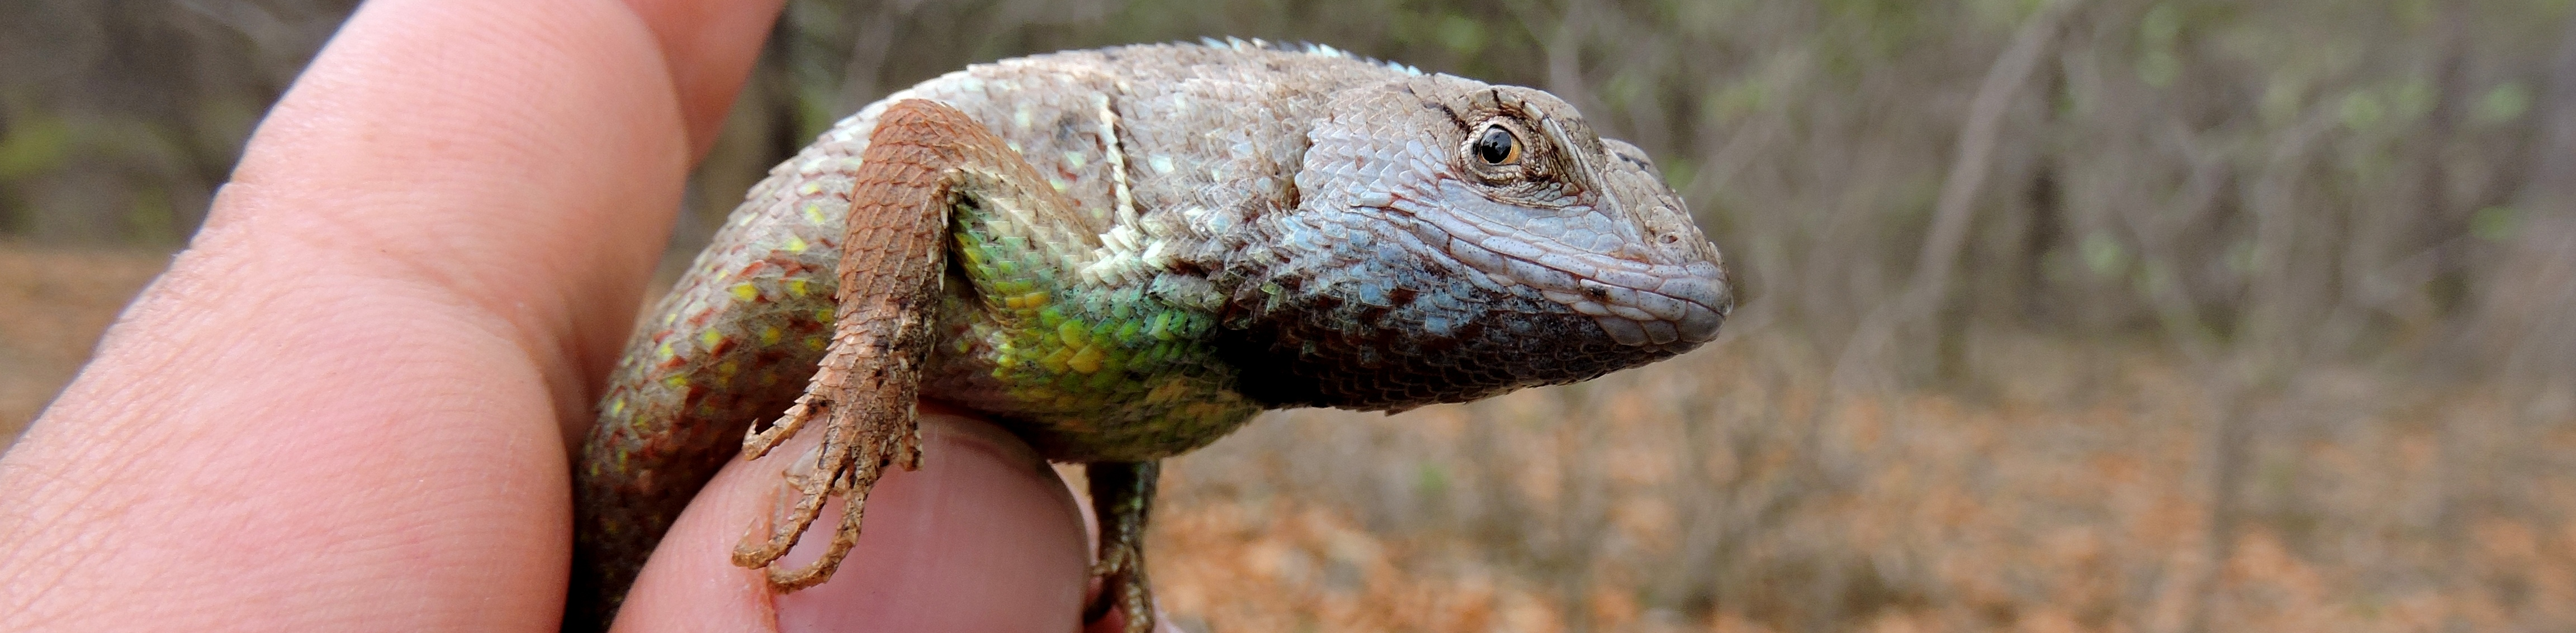
\includegraphics{lagar.jpg}
\caption{\emph{Stenocercus iridicens}}
\end{figure}

\chapter{Introducción}\label{introduccion}

La composición y estructura de la comunidad varía a lo largo de un
gradiente ambiental o a lo largo del tiempo. De esta manera, si un
ecólogo realiza un muestreo de ese gradiente, tendrá cambios en la
composición de la comunidad (las especies que la constituyen) y en la
estructura (las abundancias de las especies) (figura \ref{fig:com}).

\begin{figure}[htbp]
\centering
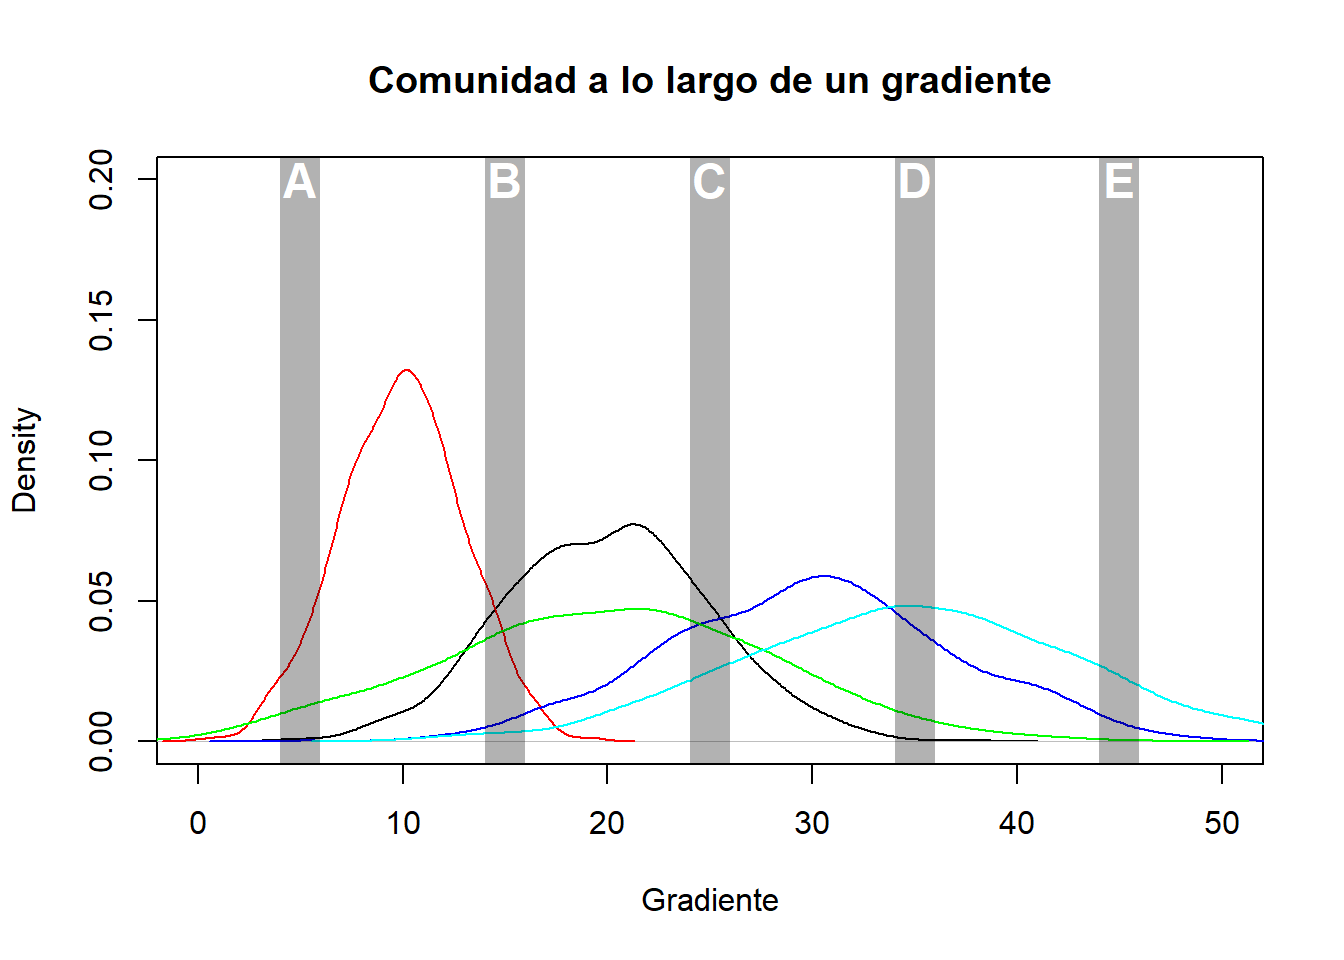
\includegraphics{Similitud_files/figure-latex/com-1.pdf}
\caption{\label{fig:com}Ejemplo de la variación de una comunidad}
\end{figure}

Como podemos ver en la figura \ref{fig:com}, en cada uno de los
transectos (representados por la línea gris), la ocurrencia de las
especies y su abundancia cambia. Por ejemplo, en la comunidad ``B''
tenemos cinco especies, la especie representada por la línea verde
alcanza su máxima abundancia, mientras que la representada por la línea
azul se encuentra con una abundancia muy baja. En la comunidad ``C''
tenemos cuatro especies pero las abundancias son diferentes a las
encontradas en la comunidad ``B''. En el caso de la comunidad ``C'', no
solo las abundancias varían sino también la ocurrencia de especies.

Los cambios en la estructura y composición de la comunidad hacen que
ciertos transectos sean más parecidos y que otros sean más distintos, en
el caso del ejemplo es clara o más o menos claras las similitudes en
cuanto a estructura y composición de las especies, sin embargo, en la
realidad es más complejo determinar a simple vista estas similitudes. A
continuación veremos que métodos se usan para cuantificar estas
similitudes.

\begin{center}\rule{0.5\linewidth}{\linethickness}\end{center}

\chapter{Similitud, disimilitud y
distancia}\label{similitud-disimilitud-y-distancia}

Pensemos que dos elementos se parecen más, cuando sus propiedades son
más parecidas, en este dos comunidades se parecerán más si su
composición y estructura es parecida. La \emph{similitud} nos permite
entonces tener un valor que define en qué medida dos comunidades se
parecen. Aunque esta información es interesante, cuando se analizan
muchas comunidades, el apreciar estas diferencias en cada par sería
complejo, por lo que interesa poder representar estas comunidades en un
plano. La graficación de las comunidades en un plano es posible si
disponemos de medidas de \textbf{distancias} entre las comunidades. Las
distancias pueden ser medidas a través de distancias simétricas (ejemplo
Euclideana, Hellinger), o a través de medidas asimétricas (medidas de
\textbf{disimilitud}), la otra cara de la similitud.

\chapter{Índices de Similitud}\label{indices-de-similitud}

¿Cuán similares son dos localidades?, vamos a calcular dos tipos de
similitudes una basada en incidencia (presencia-ausencia de especies)
(ej. Índices de \emph{Sorensen}, \emph{Jaccard} y \emph{Simpson}), y
otra basada en la abundancia \emph{Porcentaje de Similitud}. Imaginemos
que tenemos cuatro localidades (A, B, C, D) donde recogemos los datos de
densidad de cuatro especies; \emph{Tabebuia billbergii}, \emph{Geofroea
spinosa},\emph{Ceiba trichistandra} y \emph{Colicodendron scabridum},
especies características de bosques secos tropicales. Podemos introducir
datos hipotéticos de abundancia para cada especie en cada una de las
localidades.

\begin{Shaded}
\begin{Highlighting}[]
\NormalTok{dens <-}\StringTok{ }\KeywordTok{data.frame}\NormalTok{(}\DataTypeTok{T.bil =} \KeywordTok{c}\NormalTok{(}\DecValTok{1}\NormalTok{, }\DecValTok{1}\NormalTok{, }\DecValTok{2}\NormalTok{, }\DecValTok{3}\NormalTok{), }\DataTypeTok{G.spi =} \KeywordTok{c}\NormalTok{(}\DecValTok{21}\NormalTok{, }\DecValTok{8}\NormalTok{, }\DecValTok{13}\NormalTok{, }\DecValTok{5}\NormalTok{),}
                   \DataTypeTok{C.tri =} \KeywordTok{c}\NormalTok{(}\DecValTok{11}\NormalTok{, }\DecValTok{3}\NormalTok{, }\DecValTok{7}\NormalTok{, }\DecValTok{5}\NormalTok{), }\DataTypeTok{C.sca =} \KeywordTok{c}\NormalTok{(}\DecValTok{16}\NormalTok{, }\DecValTok{0}\NormalTok{, }\DecValTok{9}\NormalTok{, }\DecValTok{4}\NormalTok{))}
\KeywordTok{row.names}\NormalTok{(dens) <-}\StringTok{ }\NormalTok{LETTERS[}\DecValTok{1}\NormalTok{:}\DecValTok{4}\NormalTok{]}
\NormalTok{dens}
\end{Highlighting}
\end{Shaded}

\begin{verbatim}
##   T.bil G.spi C.tri C.sca
## A     1    21    11    16
## B     1     8     3     0
## C     2    13     7     9
## D     3     5     5     4
\end{verbatim}

Generamos un gráfico para ver cuánto se parece cada sitio (Figura
\ref{fig:NMDS}) basado en las dos primeras especies.

\begin{Shaded}
\begin{Highlighting}[]
\KeywordTok{par}\NormalTok{(}\DataTypeTok{mar=}\KeywordTok{c}\NormalTok{(}\DecValTok{4}\NormalTok{,}\DecValTok{4}\NormalTok{,}\DecValTok{1}\NormalTok{,}\DecValTok{1}\NormalTok{), }\DataTypeTok{mgp=}\KeywordTok{c}\NormalTok{(}\DecValTok{1}\NormalTok{,}\FloatTok{0.3}\NormalTok{,}\DecValTok{0}\NormalTok{), }\DataTypeTok{tcl=} \NormalTok{-}\FloatTok{0.2}\NormalTok{)}
\KeywordTok{plot}\NormalTok{(dens[,}\DecValTok{1}\NormalTok{:}\DecValTok{2}\NormalTok{], }\DataTypeTok{type =} \StringTok{"n"}\NormalTok{, }\DataTypeTok{cex.axis=}\FloatTok{0.8}\NormalTok{, }\DataTypeTok{xlim=}\KeywordTok{c}\NormalTok{(}\DecValTok{0}\NormalTok{,}\DecValTok{20}\NormalTok{), }\DataTypeTok{ylim=}\KeywordTok{c}\NormalTok{(}\DecValTok{0}\NormalTok{,}\DecValTok{25}\NormalTok{)) }
\KeywordTok{text}\NormalTok{(dens[,}\DecValTok{1}\NormalTok{:}\DecValTok{2}\NormalTok{], }\KeywordTok{row.names}\NormalTok{(dens), }\DataTypeTok{col =}\StringTok{"blue"}\NormalTok{)}
\end{Highlighting}
\end{Shaded}

\begin{figure}[htbp]
\centering
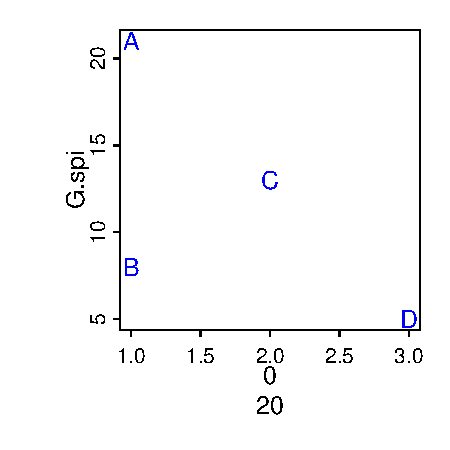
\includegraphics{Similitud_files/figure-latex/NMDS-1.pdf}
\caption{\label{fig:NMDS}Similitud de cuatro localidades hipotéticas}
\end{figure}

En la figura \ref{fig:NMDS} vemos que la composición de especies en el
sitio A es diferente de la composición del sitio D. Es decir, la
similitud entre el sitio A y D es menor que entre los otros sitios. Lo
siguiente que nos deberíamos preguntar es; ¿qué tan similares son los
dos sitios?

\section{Índices cualitativos}\label{indices-cualitativos}

Los índices cualitativos son una medida que nos permite evaluar la
similitud entre comunidades basados en presencia-ausencia de especies. A
continuación veremos tres diferentes índices:

\begin{quote}
\[S_s= \frac{(2c)}{(a+b+2c)}\] Índice de Sorensen

\[S_s= \frac{(c)}{(a+b+c)}\] Índice de Jaccard

\[S_s= \frac{(c)}{c+min(a+b)}\] Índice de Simpson
\end{quote}

Donde \emph{c} es el número de especies en común entre los dos sitios,
\emph{a} y \emph{b} son el número de especies únicas en cada sitio. Las
diferencias entre estos índices radica en la importancia que se le da a
cada componente, en el caso del índice de Sorensen las especies
compartidas tienen una gran importancia, por eso es multiplicada por
dos. En el caso del índice de Simpson, es un índice usado cuando hay
diferencias muy altas entre pares de comunidades, así restamos el peso
obteniendo el valor mínimo de entre a y b.

Para calcular estos índices entre los sitios A y B necesitamos definir
el número de especies compartidas y luego el número de especies únicas
de los dos sitios.

\begin{Shaded}
\begin{Highlighting}[]
\NormalTok{comp <-}\StringTok{ }\NormalTok{dens}
\NormalTok{comp[comp>}\DecValTok{0}\NormalTok{] <-}\StringTok{ }\DecValTok{1} \CommentTok{#Generamos una matriz de presencia ausencia}
\NormalTok{comp}
\end{Highlighting}
\end{Shaded}

\begin{verbatim}
##   T.bil G.spi C.tri C.sca
## A     1     1     1     1
## B     1     1     1     0
## C     1     1     1     1
## D     1     1     1     1
\end{verbatim}

\begin{Shaded}
\begin{Highlighting}[]
\NormalTok{a <-}\StringTok{ }\KeywordTok{sum}\NormalTok{(}\KeywordTok{colSums}\NormalTok{(comp[}\DecValTok{1}\NormalTok{:}\DecValTok{2}\NormalTok{,])==}\DecValTok{1}\NormalTok{&comp[}\DecValTok{2}\NormalTok{,]==}\DecValTok{0}\NormalTok{)}\CommentTok{#Ocurren en A pero no en B}
\NormalTok{b <-}\StringTok{ }\KeywordTok{sum}\NormalTok{(}\KeywordTok{colSums}\NormalTok{(comp[}\DecValTok{1}\NormalTok{:}\DecValTok{2}\NormalTok{,])==}\DecValTok{1}\NormalTok{&comp[}\DecValTok{1}\NormalTok{,]==}\OtherTok{FALSE}\NormalTok{)}\CommentTok{#Ocurren en B pero no en A}
\NormalTok{c <-}\StringTok{ }\KeywordTok{sum}\NormalTok{(}\KeywordTok{colSums}\NormalTok{(comp[}\DecValTok{1}\NormalTok{:}\DecValTok{2}\NormalTok{,])==}\DecValTok{2}\NormalTok{) }\CommentTok{#ocurren en A y B}

\NormalTok{a;b;c}
\end{Highlighting}
\end{Shaded}

\begin{verbatim}
## [1] 1
\end{verbatim}

\begin{verbatim}
## [1] 0
\end{verbatim}

\begin{verbatim}
## [1] 3
\end{verbatim}

Ahora obtenemos el valor de similitud entre los dos primeros sitios (A y
B).

\begin{Shaded}
\begin{Highlighting}[]
\NormalTok{Sor <-}\StringTok{ }\NormalTok{(}\DecValTok{2}\NormalTok{*c)/(a+b+(}\DecValTok{2}\NormalTok{*c))}
\NormalTok{Jac <-}\StringTok{ }\NormalTok{c/(a+b+c)}
\NormalTok{Sim <-}\StringTok{ }\NormalTok{c/c+}\KeywordTok{min}\NormalTok{(a,b)}

\NormalTok{Sor; Jac; Sim}
\end{Highlighting}
\end{Shaded}

\begin{verbatim}
## [1] 0.8571429
\end{verbatim}

\begin{verbatim}
## [1] 0.75
\end{verbatim}

\begin{verbatim}
## [1] 1
\end{verbatim}

Según el índice de Sorensen estos dos sitios son parecidos en un 86\%,
mientras que para el índice de Jaccard es el 75\% y para Simpson estos
dos sitios son iguales (100\%).

\section{Índices cuantitativos}\label{indices-cuantitativos}

El \emph{porcentaje de similitud} es la versión cuantitativa del índice
de Sorensen este índice está basado en datos de abundancia y es
calculado como:

\begin{quote}
\[S_s= \frac{(2W)}{A+B}\] Porcentaje de Similitud
\end{quote}

Donde; \emph{W} es la sumatoria del valor mínimo de la abundancia entre
las comunidades comparadas para cada especie. \emph{A} y \emph{B} es la
suma de las abundancias de todas las especies en cada sitio.

\begin{Shaded}
\begin{Highlighting}[]
\KeywordTok{library}\NormalTok{(knitr)}

\NormalTok{MatPS <-}\StringTok{ }\KeywordTok{rbind}\NormalTok{(dens[}\DecValTok{1}\NormalTok{:}\DecValTok{2}\NormalTok{,], }\KeywordTok{apply}\NormalTok{(dens[}\DecValTok{1}\NormalTok{:}\DecValTok{2}\NormalTok{, ], }\DecValTok{2}\NormalTok{, min))}\CommentTok{#Obtenemos el valor mínimo de cada especie}
\NormalTok{MatPS <-}\StringTok{ }\KeywordTok{data.frame}\NormalTok{(MatPS, }\DataTypeTok{Medidas=}\KeywordTok{rowSums}\NormalTok{(MatPS), }\DataTypeTok{Tipo=} \KeywordTok{c}\NormalTok{(}\StringTok{"A"}\NormalTok{, }\StringTok{"B"}\NormalTok{, }\StringTok{"W"}\NormalTok{)) }\CommentTok{#Obtenemos W,A,B}

\KeywordTok{kable}\NormalTok{(MatPS, }\DataTypeTok{caption =} \StringTok{"Medidas para obtener el porcentaje de Similitud"}\NormalTok{)}
\end{Highlighting}
\end{Shaded}

\begin{table}

\caption{\label{tab:unnamed-chunk-4}Medidas para obtener el porcentaje de Similitud}
\centering
\begin{tabular}[t]{l|r|r|r|r|r|l}
\hline
  & T.bil & G.spi & C.tri & C.sca & Medidas & Tipo\\
\hline
A & 1 & 21 & 11 & 16 & 49 & A\\
\hline
B & 1 & 8 & 3 & 0 & 12 & B\\
\hline
3 & 1 & 8 & 3 & 0 & 12 & W\\
\hline
\end{tabular}
\end{table}

\begin{Shaded}
\begin{Highlighting}[]
\NormalTok{PS <-}\StringTok{ }\NormalTok{(}\DecValTok{2}\NormalTok{*MatPS[}\DecValTok{3}\NormalTok{,}\DecValTok{5}\NormalTok{])/(MatPS[}\DecValTok{1}\NormalTok{,}\DecValTok{5}\NormalTok{]+MatPS[}\DecValTok{2}\NormalTok{,}\DecValTok{5}\NormalTok{])}
\NormalTok{PS}
\end{Highlighting}
\end{Shaded}

\begin{verbatim}
## [1] 0.3934426
\end{verbatim}

Esto significa que la comunidad A y B tienen un porcentaje de similitud
del 39\%. Los datos de los dos tipos de índices utilizados difieren
entre sí, el porcentaje de similitud utiliza no solamente la presencia
ausencia sino también la abundancia lo que podría estar reduciendo la
similitud entre sitios.

\chapter{Distancias entre sitios}\label{distancias-entre-sitios}

Cuando tenemos dos comunidades muy parecidas entre sí tendremos valores
altos de similitud, en contraposición los índices de distancia nos
mostrarán valores altos cuando dos comunidades se parecen poco. Como
habíamos mencionado anteriormente existes dos tipos de medidas de
distancia;

\begin{itemize}
\item
  aquellas calculadas a partir de los índices de similitud usualmente
  como D= 1-Similitud. Así, para los índices de incidencia (presencia -
  ausencia) se pueden usar los índices de Jacard, Simpson o Sorensen,
  mientras que para los índices cuantitativos se puede usar el
  porcentaje de similitud, este último conocido como distancia de Bray
  Curtis.
\item
  aquellas que no tienen medidas de similitud análogas, algunos de estos
  índices son; Euclidiana, Chord, Hellinger.
\end{itemize}

La \emph{distancia} entre dos muestras está dada por la diferencia entre
la abundancia y la composición de especies, como lo hemos visto esto
genera una distancia, en el caso del ejemplo la comunidad A esta más
alejada de la comunidad D que de las otras dos (figura \ref{fig:NMDS}).

\section{Distancia Euclidiana}\label{distancia-euclidiana}

Existen muchas formas de poder calcular las distancias entre estos
puntos una de las más sencillas es la distancia \emph{Euclidiana}. La
distancia euclidiana entre dos sitios es simplemente la longitud del
vector que conecta los sitios y la podemos obtener como
\(\sqrt{x^2+y^2}\), donde \emph{``x''} y \emph{``y''} son las
coordenadas (x, y) de distancia entre un par de sitios.

En nuestro caso si queremos comparar B y C tenemos que la distancia en
el eje \emph{x} es la diferencia de la abundancia de \emph{T. bilbergii}
entre el sitio B y C.

\begin{Shaded}
\begin{Highlighting}[]
\NormalTok{x <-}\StringTok{ }\NormalTok{dens[}\DecValTok{2}\NormalTok{, }\DecValTok{1}\NormalTok{] -}\StringTok{ }\NormalTok{dens[}\DecValTok{3}\NormalTok{, }\DecValTok{1}\NormalTok{]}
\end{Highlighting}
\end{Shaded}

Mientras que la distancia en el eje \emph{y} es la diferencia en la
abundancia de \emph{G. spinosa} entre el sitio B y C.

\begin{Shaded}
\begin{Highlighting}[]
\NormalTok{y <-}\StringTok{ }\NormalTok{dens[}\DecValTok{2}\NormalTok{, }\DecValTok{2}\NormalTok{] -}\StringTok{ }\NormalTok{dens[}\DecValTok{3}\NormalTok{, }\DecValTok{2}\NormalTok{]}
\end{Highlighting}
\end{Shaded}

Ahora obtenemos las distancias entre los dos sitios

\begin{Shaded}
\begin{Highlighting}[]
\KeywordTok{sqrt}\NormalTok{(x^}\DecValTok{2} \NormalTok{+}\StringTok{ }\NormalTok{y^}\DecValTok{2}\NormalTok{)}
\end{Highlighting}
\end{Shaded}

\begin{verbatim}
## [1] 5.09902
\end{verbatim}

Pero como en \emph{R} todo es sencillo podemos utilizar la función
\emph{dist}

\begin{Shaded}
\begin{Highlighting}[]
\KeywordTok{dist}\NormalTok{(dens[,}\DecValTok{1}\NormalTok{:}\DecValTok{2}\NormalTok{])}
\end{Highlighting}
\end{Shaded}

\begin{verbatim}
##           A         B         C
## B 13.000000                    
## C  8.062258  5.099020          
## D 16.124515  3.605551  8.062258
\end{verbatim}

Si bien este cálculo es sencillo con dos especies, si tenemos que
calcular la distancia para una comunidad con más de tres especies los
cálculos son tediosos y largos. Para calcular la distancia
\emph{Euclidiana} entre pares de sitios con \emph{R} especies utilizamos
la siguiente ecuación:

\begin{quote}
\[D_E = \sqrt{\sum_{i=l}^R (x_{ai} - x_{bi})^2}\] Distancia Euclidiana
\end{quote}

\subsection{Efecto de doble-ceros y
abundancia}\label{efecto-de-doble-ceros-y-abundancia}

Aunque la distancia Euclidiana es fácilmente interpretable, es poco
usado en análisis biológicos. Normalmente los datos de comunidad están
caracterizados por una gran cantidad de ceros (especies no encontradas
en determinados sitios), el cálculo de la distancia Euclidiana
incrementa la similitud entre comunidades que presentan ceros en la
misma especie.

\begin{table}

\caption{\label{tab:unnamed-chunk-9}Efecto del doble cero}
\centering
\begin{tabular}[t]{r|r|r|r|r|r}
\hline
spp1 & spp2 & spp3 & sp4 & spp5 & spp6\\
\hline
1 & 1 & 0 & 0 & 0 & 0\\
\hline
0 & 1 & 1 & 1 & 1 & 0\\
\hline
0 & 0 & 0 & 0 & 1 & 1\\
\hline
\end{tabular}
\end{table}

Según los datos mostrados en la tabla tendríamos que hay un gradiente,
la primera comunidad comparte una especie con la comunidad dos y la
comunidad dos comparte una especie con la comunidad tres. Los índices
deberían permitir recuperar ese gradiente, veamos lo que pasa.

\begin{Shaded}
\begin{Highlighting}[]
\KeywordTok{library}\NormalTok{(vegan)}
\end{Highlighting}
\end{Shaded}

\begin{verbatim}
## Loading required package: permute
\end{verbatim}

\begin{verbatim}
## Loading required package: lattice
\end{verbatim}

\begin{verbatim}
## This is vegan 2.5-2
\end{verbatim}

\begin{Shaded}
\begin{Highlighting}[]
\KeywordTok{vegdist}\NormalTok{(dcMat, }\StringTok{"euclidean"}\NormalTok{)}
\end{Highlighting}
\end{Shaded}

\begin{verbatim}
##   1 2
## 2 2  
## 3 2 2
\end{verbatim}

Como vemos, en el caso del ejemplo el doble cero de la comunidad uno y
tres generan una mayor similitud, por lo que las tres comunidades son
mostradas a igual distancia. Esto no debería ser un problema, si el cero
realmente nos da información, pero en el caso de datos biológicos la
razón de tener ese cero puede deberse a varias razones, por lo que
realmente el cero no es informativo. En otros casos, normalmente en
datos abióticos, el cero implica la ausencia de algo, por ejemplo tener
cero mg de un contaminante es una información. De esta forma la
distancia Euclidiana es usada sobre todo para interpretar datos
ambientales.

Otra característica importante de la distancia euclidiana es que está
fuertemente impactada por la diferencia de abundancias, recordemos que
la diferencia de abundancias esta elevada al cuadrado, de esta forma la
distancia entre dos comunidades puede estar marcada por la diferencia en
abundancias más que por la diferencia en presencia de especies.

\begin{Shaded}
\begin{Highlighting}[]
\NormalTok{dcMat2 <-}\StringTok{ }\KeywordTok{data.frame}\NormalTok{(}\DataTypeTok{spp1=}\KeywordTok{c}\NormalTok{(}\DecValTok{0}\NormalTok{,}\DecValTok{1}\NormalTok{,}\DecValTok{0}\NormalTok{),}\DataTypeTok{spp2=}\KeywordTok{c}\NormalTok{(}\DecValTok{1}\NormalTok{,}\DecValTok{0}\NormalTok{,}\DecValTok{8}\NormalTok{),}
                    \DataTypeTok{spp3=}\KeywordTok{c}\NormalTok{(}\DecValTok{1}\NormalTok{,}\DecValTok{0}\NormalTok{,}\DecValTok{7}\NormalTok{))}

\KeywordTok{kable}\NormalTok{(dcMat2, }\DataTypeTok{caption =} \StringTok{"Efecto de la abundancia"}\NormalTok{)}
\end{Highlighting}
\end{Shaded}

\begin{table}

\caption{\label{tab:unnamed-chunk-11}Efecto de la abundancia}
\centering
\begin{tabular}[t]{r|r|r}
\hline
spp1 & spp2 & spp3\\
\hline
0 & 1 & 1\\
\hline
1 & 0 & 0\\
\hline
0 & 8 & 7\\
\hline
\end{tabular}
\end{table}

\begin{Shaded}
\begin{Highlighting}[]
\KeywordTok{vegdist}\NormalTok{(dcMat2, }\StringTok{"euclidean"}\NormalTok{)}
\end{Highlighting}
\end{Shaded}

\begin{verbatim}
##           1         2
## 2  1.732051          
## 3  9.219544 10.677078
\end{verbatim}

Como vemos la comunidad uno se encuentra más cercana a la comunidad dos
que a la tres. La distancia de la comunidad uno a la tres es de 9.21,
aunque comparten dos especies la diferencia en abundancias es muy
marcada. Por otro lado, la comunidad uno tiene una distancia de 1.73 a
la comunidad dos, esta menor distancia se da aunque no comparten ninguna
especie.

\section{Distancia Bray-Curtis}\label{distancia-bray-curtis}

Existen otras formas de medir distancias entre dos localidades. En
ecología una de las distancias más utilizada es la distancia de
\emph{Bray-Curtis}, como mencionamos anteriormente esta distancia es el
opuesto del porcentaje de similitud, que a su vez es la versión de
abundancia del índice de Sorensen. Esta distancia es calculada como:

\begin{quote}
\[D_{BC} = \sum_{i=l}^R \frac{(x_{ai} - x_{bi})}{(x_{ai} + x_{bi})}\]
Distancia de Bray-Curtis
\end{quote}

La distancia \emph{Bray-Curtis} se refiere a la diferencia total en la
abundancia de especies entre dos sitios, dividido para la abundancia
total en cada sitio. La distancia Bray-Curtis tiende a resultar más
intuitiva debido a que las especies comunes y raras tienen pesos
relativamente similares, mientras que la distancia euclidiana depende en
mayor medida de las especies más abundantes. Esto sucede porque las
distancias euclidianas se basan en diferencias al cuadrado, mientras que
Bray-Curtis utiliza diferencias absolutas. El elevar un número al
cuadrado siempre amplifica la importancia de los valores más grandes. En
la figura \ref{fig:bray} se compara gráficos basados en distancias
euclidianas y Bray-Curtis de los mismos datos.

Como se había comentado, es virtualmente imposible representar una
distancia en más de tres dimensiones (cada especie es una dimensión).
Una forma sencilla de mostrar distancias para tres o más especies es
crear un gráfico de dos dimensiones, intentando organizar todos los
sitios para que las distancias sean aproximadamente las correctas. Está
claro que esto es una aproximación nunca estas serán exactas. Una
técnica que intenta crear un arreglo aproximado es escalamiento
multidimensional no métrico (NMDS).

La función de escalamiento multidimensional no-métrico está en el
paquete \texttt{vegan}. Aquí mostramos las distancias euclidianas entre
sitios (Figura \ref{fig:bray}a) y las distancias de Bray-Curtis (Figura
\ref{fig:bray}b).

\begin{Shaded}
\begin{Highlighting}[]
\KeywordTok{library}\NormalTok{(vegan) }

\CommentTok{#Distancia Euclidiana}
\NormalTok{mdsE <-}\StringTok{ }\KeywordTok{metaMDS}\NormalTok{(dcMat, }\DataTypeTok{distance =} \StringTok{"euc"}\NormalTok{, }\DataTypeTok{autotransform =} \OtherTok{FALSE}\NormalTok{, }\DataTypeTok{trace =} \DecValTok{0}\NormalTok{) }
\CommentTok{#Distancia de Bray-Curtis}
\NormalTok{mdsB <-}\StringTok{ }\KeywordTok{metaMDS}\NormalTok{(dcMat, }\DataTypeTok{distance =} \StringTok{"bray"}\NormalTok{, }\DataTypeTok{autotransform =} \OtherTok{FALSE}\NormalTok{, }\DataTypeTok{trace =} \DecValTok{0}\NormalTok{) }
\end{Highlighting}
\end{Shaded}

\begin{Shaded}
\begin{Highlighting}[]
\KeywordTok{par}\NormalTok{(}\DataTypeTok{mfcol=}\KeywordTok{c}\NormalTok{(}\DecValTok{1}\NormalTok{,}\DecValTok{2}\NormalTok{), }\DataTypeTok{oma=}\KeywordTok{c}\NormalTok{(}\DecValTok{1}\NormalTok{,}\DecValTok{1}\NormalTok{,}\DecValTok{1}\NormalTok{,}\DecValTok{1}\NormalTok{), }\DataTypeTok{mar=}\KeywordTok{c}\NormalTok{(}\DecValTok{4}\NormalTok{,}\DecValTok{4}\NormalTok{,}\DecValTok{1}\NormalTok{,}\DecValTok{1}\NormalTok{),}
    \DataTypeTok{mgp=}\KeywordTok{c}\NormalTok{(}\DecValTok{1}\NormalTok{,}\FloatTok{0.3}\NormalTok{,}\DecValTok{0}\NormalTok{), }\DataTypeTok{tcl=} \NormalTok{-}\FloatTok{0.2}\NormalTok{)}

\KeywordTok{plot}\NormalTok{(mdsE, }\DataTypeTok{display =} \StringTok{"sites"}\NormalTok{, }
     \DataTypeTok{type =} \StringTok{"text"}\NormalTok{,}\DataTypeTok{main=}\StringTok{"a)Euclidiana"}\NormalTok{, }
     \DataTypeTok{cex.axis=} \FloatTok{0.7}\NormalTok{, }\DataTypeTok{cex.main=}\FloatTok{0.75}\NormalTok{, }\DataTypeTok{cex.lab=}\FloatTok{0.7}\NormalTok{)}

\KeywordTok{plot}\NormalTok{(mdsB, }\DataTypeTok{display =} \StringTok{"sites"}\NormalTok{, }\DataTypeTok{type =} \StringTok{"text"}\NormalTok{, }
     \DataTypeTok{main=}\StringTok{"b)Bray-Curtis"}\NormalTok{, }
     \DataTypeTok{cex.axis=} \FloatTok{0.7}\NormalTok{, }\DataTypeTok{cex.main=}\FloatTok{0.75}\NormalTok{, }\DataTypeTok{cex.lab=}\FloatTok{0.7}\NormalTok{)}
\end{Highlighting}
\end{Shaded}

\begin{figure}[htbp]
\centering
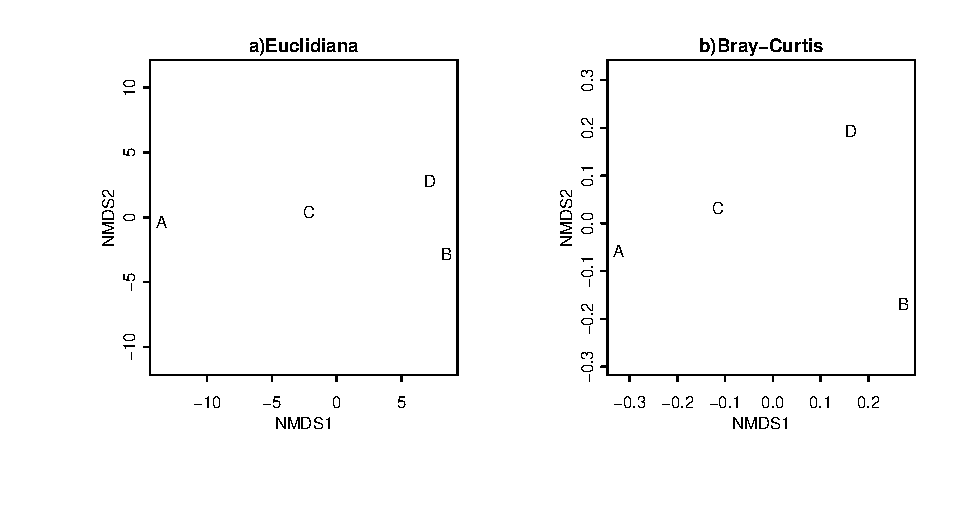
\includegraphics{Similitud_files/figure-latex/bray-1.pdf}
\caption{\label{fig:bray}Arreglo de las parcelas en distancias
multidimensionales no métricas (NMDS). Estas dos figuras muestran los
mismos datos en bruto, pero las distancias euclidianas tienden a
enfatizar las diferencias debidas a las especies más abundantes,
mientras que Bray-Curtis no lo hace.}
\end{figure}

Como podemos apreciar en el caso del ejemplo, la distancia de
Bray-Curtis recupera la idea de un gradiente entre las comunidades,
desde la comunidad uno a la tres. En el caso de la distancia Euclidiana
la comunidad dos y tres se encuentran a igual distancia de la comunidad
uno, como un efecto del doble cero.

\chapter{Transformación y Estandarización de
datos}\label{transformacion-y-estandarizacion-de-datos}

Cuando trabajamos con datos multivariantes cabe la posibilidad de que
los datos dentro de esta matriz tengan diferencias de magnitud
importantes. Como vimos antes el cálculo de distancia entre los sitios
puede verse fuertemente afectado por la magnitud de sus diferencias.

En el ejemplo que mostramos en el inicio, las similitudes entre
comunidades basadas en las dos primeras especies, las diferencias entre
las comunidades depende de la escala de medición (los valores de los
ejes), y sobre cómo medimos la distancia a través del espacio
multivariado \citep{Stevens2009}.

De esta forma, las diferencias entre sitios son dependientes de la
abundancia de cada especie. En el caso de \emph{G. spinosa} su eje varía
entre 5 y 21, mientras que para \emph{T. billbergii} varía entre 1 y 3
(Figura \ref{fig:NMDS2}a). Veamos ahora que sucede con las similitud si
incremento la abundancia de \emph{T. billbergii} (Figura
\ref{fig:NMDS2}b).

\begin{Shaded}
\begin{Highlighting}[]
\KeywordTok{par}\NormalTok{(}\DataTypeTok{mar=}\KeywordTok{c}\NormalTok{(}\DecValTok{4}\NormalTok{,}\DecValTok{4}\NormalTok{,}\DecValTok{1}\NormalTok{,}\DecValTok{1}\NormalTok{), }\DataTypeTok{mgp=}\KeywordTok{c}\NormalTok{(}\DecValTok{1}\NormalTok{,}\FloatTok{0.3}\NormalTok{,}\DecValTok{0}\NormalTok{), }\DataTypeTok{mfcol=}\KeywordTok{c}\NormalTok{(}\DecValTok{1}\NormalTok{,}\DecValTok{2}\NormalTok{), }\DataTypeTok{tcl=} \NormalTok{-}\FloatTok{0.2}\NormalTok{)}
\NormalTok{dens1 <-}\StringTok{ }\NormalTok{dens}
\NormalTok{dens1$T.bil <-}\StringTok{ }\NormalTok{dens1$T.bil*}\DecValTok{100}
\KeywordTok{plot}\NormalTok{(dens[,}\DecValTok{1}\NormalTok{:}\DecValTok{2}\NormalTok{], }\DataTypeTok{type =} \StringTok{"n"}\NormalTok{, }\DataTypeTok{cex.axis=}\FloatTok{0.8}\NormalTok{, }\DataTypeTok{xlim=}\KeywordTok{c}\NormalTok{(}\DecValTok{0}\NormalTok{,}\DecValTok{30}\NormalTok{), }\DataTypeTok{ylim=}\KeywordTok{c}\NormalTok{(}\DecValTok{0}\NormalTok{,}\DecValTok{30}\NormalTok{), }\DataTypeTok{main=}\StringTok{"a."}\NormalTok{) }
\KeywordTok{text}\NormalTok{(dens[,}\DecValTok{1}\NormalTok{:}\DecValTok{2}\NormalTok{], }\KeywordTok{row.names}\NormalTok{(dens), }\DataTypeTok{col =}\StringTok{"blue"}\NormalTok{)}

\KeywordTok{plot}\NormalTok{(dens1[,}\DecValTok{1}\NormalTok{:}\DecValTok{2}\NormalTok{], }\DataTypeTok{type =} \StringTok{"n"}\NormalTok{, }\DataTypeTok{cex.axis=}\FloatTok{0.8}\NormalTok{, }\DataTypeTok{ylim=}\KeywordTok{c}\NormalTok{(}\DecValTok{0}\NormalTok{,}\DecValTok{300}\NormalTok{), }\DataTypeTok{main=}\StringTok{"b."}\NormalTok{) }
\KeywordTok{text}\NormalTok{(dens1[,}\DecValTok{1}\NormalTok{:}\DecValTok{2}\NormalTok{], }\KeywordTok{row.names}\NormalTok{(dens1), }\DataTypeTok{col =}\StringTok{"blue"}\NormalTok{)}
\end{Highlighting}
\end{Shaded}

\begin{figure}[htbp]
\centering
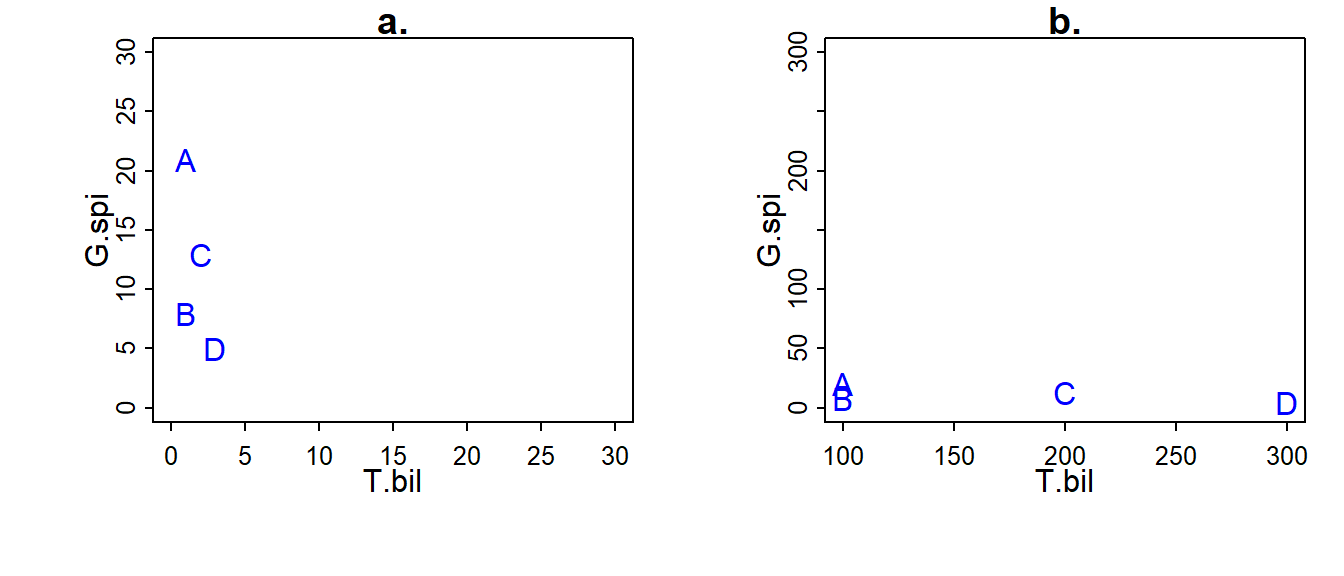
\includegraphics{Similitud_files/figure-latex/NMDS2-1.pdf}
\caption{\label{fig:NMDS2}Distancias de cuatro localidades hipotéticas}
\end{figure}

Como vemos en la figura \ref{fig:NMDS2} las distancias entre cada uno de
los sitios cambio cuando incremento la abundancia de \emph{T. bilbergi},
aunque este incremento fue proporcional. Una forma de corregir esta
distorsión es calcular la densidad relativa de cada especie, de esta
forma cada especie variará entre 0 y 1 \citep{Stevens2009}. Cuando nos
referimos a densidad relativa hablamos de la densidad de una especie con
referencia a algo, en este caso con relación a la abundancia de
individuos de la misma especie en otros sitios.

Para calcular la densidad relativa dividimos la abundancia de cada
especie para la suma total de los individuos de las especies en esa
muestra.

\begin{Shaded}
\begin{Highlighting}[]
\NormalTok{dens[,}\DecValTok{1}\NormalTok{]/}\KeywordTok{sum}\NormalTok{(dens[,}\DecValTok{1}\NormalTok{])}
\end{Highlighting}
\end{Shaded}

\begin{verbatim}
## [1] 0.1428571 0.1428571 0.2857143 0.4285714
\end{verbatim}

\begin{Shaded}
\begin{Highlighting}[]
\NormalTok{dens1[,}\DecValTok{1}\NormalTok{]/}\KeywordTok{sum}\NormalTok{(dens1[,}\DecValTok{1}\NormalTok{])}
\end{Highlighting}
\end{Shaded}

\begin{verbatim}
## [1] 0.1428571 0.1428571 0.2857143 0.4285714
\end{verbatim}

Ahora podemos ver cómo \emph{T. billbergii} varía en su abundancia en
los cuatro sitios. El sitio A y B tienen el 14\% de individuos mientras
que el D tiene el 42\% de los individuos de esta especie.
Interesantemente, no hay diferencias en las proporciones entre las dos
medidas que tenemos. ¿Qué pasó con las distancias?

\begin{figure}[htbp]
\centering
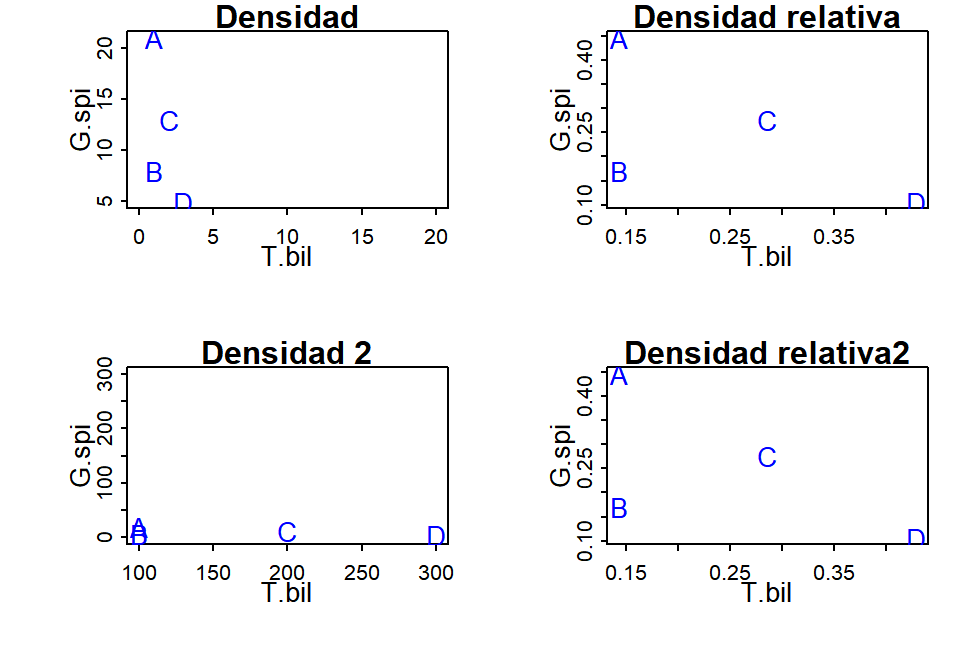
\includegraphics{Similitud_files/figure-latex/NMDS3-1.pdf}
\caption{\label{fig:NMDS3}Distancias de cuatro localidades hipotéticas}
\end{figure}

En la figura \ref{fig:NMDS3} podemos apreciar que no hay diferencias
entre las dos densidades cuando estoy usando la densidad relativa. Pero
¿Qué implicaciones biológicas tiene el usar las densidades relativas
para calcular la distancia entre sitios?

Cuando usamos las densidades relativas estamos dando el mismo peso a
todas las especies. En un ecosistema con una especie dominante y varias
subordinadas, al usar la densidad relativa estoy eliminando esa
dominancia. Es importante tener claro este punto, ya que las
interpretaciones que puedo hacer con los datos de densidad y densidad
relativa son distintos.

\section{Transformación de datos}\label{transformacion-de-datos}

Como vemos la magnitud de las diferencias entre las variables tiene un
impacto sobre el cálculo de la distancia, por lo que nos interesa poder
manejar el efecto de esas diferencias, para lo cual desarrollamos una
transformación.

La transformación de datos implica una modificación de los datos brutos
a través de una ecuación algebraica. La transformación de datos implica
una modificación independientemente para cada dato, no existe influencia
del resto de datos.

\begin{table}

\caption{\label{tab:unnamed-chunk-15}Comunidad de macroinvertebrados acuáticos}
\centering
\begin{tabular}[t]{l|r|r|r|r|r|r|r|r|r|r|r}
\hline
LOCALIDAD & Allu & Atop & Atri & Baet & Bezz & Blep & Cera & Chel & Chim & Chir & Cole\\
\hline
Bo-1 & 0 & 0 & 0 & 6 & 0 & 1 & 0 & 1 & 3 & 18 & 4\\
\hline
Bo-2 & 0 & 0 & 0 & 3 & 0 & 0 & 0 & 0 & 1 & 9 & 0\\
\hline
Bo-3 & 0 & 0 & 0 & 6 & 0 & 0 & 1 & 1 & 1 & 9 & 0\\
\hline
BP-1 & 0 & 3 & 0 & 81 & 0 & 0 & 0 & 0 & 0 & 27 & 0\\
\hline
BP-2 & 0 & 0 & 0 & 9 & 0 & 0 & 0 & 0 & 2 & 0 & 0\\
\hline
BP-3 & 0 & 0 & 0 & 54 & 0 & 0 & 1 & 0 & 0 & 9 & 0\\
\hline
Pa-1 & 1 & 0 & 0 & 984 & 0 & 0 & 0 & 0 & 0 & 81 & 0\\
\hline
Pa-2 & 0 & 0 & 0 & 15 & 0 & 0 & 0 & 0 & 1 & 9 & 0\\
\hline
Pa-3 & 0 & 0 & 0 & 93 & 1 & 0 & 0 & 0 & 0 & 18 & 0\\
\hline
Ur-1 & 0 & 0 & 0 & 6 & 0 & 0 & 0 & 0 & 0 & 855 & 0\\
\hline
Ur-2 & 0 & 0 & 1 & 12 & 0 & 0 & 0 & 1 & 0 & 9 & 0\\
\hline
Ur-3 & 0 & 0 & 0 & 0 & 10 & 0 & 0 & 0 & 0 & 27 & 0\\
\hline
\end{tabular}
\end{table}

En la tabla anterior podemos ver que la comunidad está compuesta por un
par de especies dominantes y varias especies raras.

Al transformar los datos evitamos que las especies dominantes definan el
cálculo de la distancia.

Existen varias posibilidades para transformar los datos, por lo que
definir que función utilizar es importante. Cada tipo de transformación
produce resultados distintos por lo que debemos utilizarlas con
precaución.

La transformación más sencilla o menos intensa es la raíz cuadrada,
mientras que el logaritmo es la transformación más intensa, podríamos
utilizar la raíz cuarta como una función intermedia. La raíz cuadrada la
utilizaríamos cuando tenemos diferencias con variaciones de una magnitud
de diferencia (entre decenas y centenas), mientras que la transformación
logarítmica la haríamos con comunidades donde hay más de una magnitud de
diferencia (entre decenas y miles).

Aunque hay muchos autores que aconsejan realizar transformaciones hay
que ser conscientes de lo que estamos haciendo, transformaciones muy
fuertes en una matriz con pocas diferencias pueden hacer que, por
ejemplo, las especies raras tengan igual peso que las dominantes, ¿esto
es lo que queremos?

\textbf{Recuerde: las diferentes transformaciones tienen
interpretaciones biológicas distintas. Debemos ser conscientes de lo que
estamos haciendo y de su posterior interpretación biológica.}

Veamos un ejemplo:

\begin{Shaded}
\begin{Highlighting}[]
\KeywordTok{set.seed}\NormalTok{(}\DecValTok{4}\NormalTok{)}
\NormalTok{aves<-}\StringTok{ }\KeywordTok{data.frame}\NormalTok{(}\DataTypeTok{sp1=} \KeywordTok{sample}\NormalTok{(}\DecValTok{1}\NormalTok{:}\DecValTok{90}\NormalTok{, }\DecValTok{10}\NormalTok{), }\DataTypeTok{sp2=} \KeywordTok{sample}\NormalTok{(}\DecValTok{100}\NormalTok{:}\DecValTok{250}\NormalTok{, }\DecValTok{10}\NormalTok{))}

\NormalTok{insectos<-}\StringTok{ }\KeywordTok{data.frame}\NormalTok{(}\DataTypeTok{sp1=} \KeywordTok{sample}\NormalTok{(}\DecValTok{5}\NormalTok{:}\DecValTok{99}\NormalTok{, }\DecValTok{10}\NormalTok{), }\DataTypeTok{sp2=} \KeywordTok{sample}\NormalTok{(}\DecValTok{1000}\NormalTok{:}\DecValTok{2500}\NormalTok{, }\DecValTok{10}\NormalTok{))}

\NormalTok{##¿Qué pasa cuando transformamos?}
\NormalTok{aveT <-}\StringTok{ }\KeywordTok{round}\NormalTok{(}\KeywordTok{cbind}\NormalTok{(aves, }\KeywordTok{sqrt}\NormalTok{(aves),}\KeywordTok{log}\NormalTok{(aves)),}\DecValTok{2}\NormalTok{)}
\KeywordTok{colnames}\NormalTok{(aveT) <-}\StringTok{ }\KeywordTok{paste}\NormalTok{(}\KeywordTok{rep}\NormalTok{(}\KeywordTok{c}\NormalTok{(}\StringTok{"sp1"}\NormalTok{, }\StringTok{"sp2"}\NormalTok{), }\DecValTok{3}\NormalTok{), }\KeywordTok{c}\NormalTok{(}\StringTok{""}\NormalTok{,}\StringTok{""}\NormalTok{,}\StringTok{"sqrt"}\NormalTok{, }\StringTok{"sqrt"}\NormalTok{, }\StringTok{"log"}\NormalTok{, }\StringTok{"log"}\NormalTok{), }\DataTypeTok{sep=}\StringTok{"."}\NormalTok{)}

\KeywordTok{kable}\NormalTok{(aveT, }\DataTypeTok{caption =} \StringTok{"Efecto de la transformación. Pequeñas diferencias"}\NormalTok{)}
\end{Highlighting}
\end{Shaded}

\begin{table}

\caption{\label{tab:unnamed-chunk-16}Efecto de la transformación. Pequeñas diferencias}
\centering
\begin{tabular}[t]{r|r|r|r|r|r}
\hline
sp1. & sp2. & sp1.sqrt & sp2.sqrt & sp1.log & sp2.log\\
\hline
53 & 213 & 7.28 & 14.59 & 3.97 & 5.36\\
\hline
1 & 142 & 1.00 & 11.92 & 0.00 & 4.96\\
\hline
26 & 114 & 5.10 & 10.68 & 3.26 & 4.74\\
\hline
25 & 241 & 5.00 & 15.52 & 3.22 & 5.48\\
\hline
70 & 161 & 8.37 & 12.69 & 4.25 & 5.08\\
\hline
23 & 166 & 4.80 & 12.88 & 3.14 & 5.11\\
\hline
61 & 240 & 7.81 & 15.49 & 4.11 & 5.48\\
\hline
76 & 184 & 8.72 & 13.56 & 4.33 & 5.21\\
\hline
78 & 237 & 8.83 & 15.39 & 4.36 & 5.47\\
\hline
6 & 208 & 2.45 & 14.42 & 1.79 & 5.34\\
\hline
\end{tabular}
\end{table}

\begin{Shaded}
\begin{Highlighting}[]
\NormalTok{insT <-}\StringTok{ }\KeywordTok{round}\NormalTok{(}\KeywordTok{cbind}\NormalTok{(insectos, }\KeywordTok{sqrt}\NormalTok{(insectos),}\KeywordTok{log}\NormalTok{(insectos)),}\DecValTok{2}\NormalTok{) }
\KeywordTok{colnames}\NormalTok{(insT) <-}\StringTok{ }\KeywordTok{paste}\NormalTok{(}\KeywordTok{rep}\NormalTok{(}\KeywordTok{c}\NormalTok{(}\StringTok{"sp1"}\NormalTok{, }\StringTok{"sp2"}\NormalTok{), }\DecValTok{3}\NormalTok{), }\KeywordTok{c}\NormalTok{(}\StringTok{""}\NormalTok{,}\StringTok{""}\NormalTok{,}\StringTok{"sqrt"}\NormalTok{, }\StringTok{"sqrt"}\NormalTok{, }\StringTok{"log"}\NormalTok{, }\StringTok{"log"}\NormalTok{), }\DataTypeTok{sep=}\StringTok{"."}\NormalTok{)}

\KeywordTok{kable}\NormalTok{(insT, }\DataTypeTok{caption =} \StringTok{"Efecto de la transformación, Grandes diferencias"}\NormalTok{)}
\end{Highlighting}
\end{Shaded}

\begin{table}

\caption{\label{tab:unnamed-chunk-16}Efecto de la transformación, Grandes diferencias}
\centering
\begin{tabular}[t]{r|r|r|r|r|r}
\hline
sp1. & sp2. & sp1.sqrt & sp2.sqrt & sp1.log & sp2.log\\
\hline
72 & 1851 & 8.49 & 43.02 & 4.28 & 7.52\\
\hline
98 & 1358 & 9.90 & 36.85 & 4.58 & 7.21\\
\hline
52 & 2316 & 7.21 & 48.12 & 3.95 & 7.75\\
\hline
50 & 1980 & 7.07 & 44.50 & 3.91 & 7.59\\
\hline
64 & 1722 & 8.00 & 41.50 & 4.16 & 7.45\\
\hline
79 & 2452 & 8.89 & 49.52 & 4.37 & 7.80\\
\hline
47 & 1687 & 6.86 & 41.07 & 3.85 & 7.43\\
\hline
94 & 1929 & 9.70 & 43.92 & 4.54 & 7.56\\
\hline
49 & 1579 & 7.00 & 39.74 & 3.89 & 7.36\\
\hline
96 & 1009 & 9.80 & 31.76 & 4.56 & 6.92\\
\hline
\end{tabular}
\end{table}

\section{Estandarización de los
datos}\label{estandarizacion-de-los-datos}

La estandarización de los datos permite modificar las variables
transformándolas en unidades de desviación típica, lo que nos permite
comparar entre valores de distribuciones normales diferentes, o de
valores diferentes.

La estandarización o tipificación se lo realiza restando a cada valor el
valor medio de la variable y dividiendo para la desviación estándar.

\begin{Shaded}
\begin{Highlighting}[]
\NormalTok{avesE <-}\StringTok{ }\NormalTok{(aves[,}\DecValTok{1}\NormalTok{]-}\KeywordTok{mean}\NormalTok{(aves[,}\DecValTok{1}\NormalTok{]))/}\KeywordTok{sd}\NormalTok{(aves[,}\DecValTok{1}\NormalTok{])}
\NormalTok{avesE}
\end{Highlighting}
\end{Shaded}

\begin{verbatim}
##  [1]  0.3819546 -1.4073822 -0.5471241 -0.5815345  0.9669301 -0.6503551
##  [7]  0.6572372  1.1733920  1.2422126 -1.2353306
\end{verbatim}

\begin{Shaded}
\begin{Highlighting}[]
\KeywordTok{round}\NormalTok{(}\KeywordTok{mean}\NormalTok{(avesE),}\DecValTok{1}\NormalTok{);}\KeywordTok{sd}\NormalTok{(avesE) }
\end{Highlighting}
\end{Shaded}

\begin{verbatim}
## [1] 0
\end{verbatim}

\begin{verbatim}
## [1] 1
\end{verbatim}

Como vemos las variables estandarizadas tienen como propiedad que la
desviación estándar es 1 y la media es 0.

\begin{center}\rule{0.5\linewidth}{\linethickness}\end{center}

\chapter{Ejercicio práctico}\label{ejercicio-practico}

\begin{center}\rule{0.5\linewidth}{\linethickness}\end{center}

Una de las preguntas básicas de un ecólogo es saber ¿Cómo de diferentes
son dos comunidades?. Como hemos visto existen varias decisiones que los
investigadores debemos tomar, estas decisiones afectan directamente a
los resultados que podemos obtener y por ende a las conclusiones
biológicas que obtenemos de este análisis.

El presente ejercicio evaluaremos como las diferentes decisiones que
tomamos entorno al procesamiento de datos afectan nuestras medidas de
similitud, y cuáles son las conclusiones biológicas que obtenemos con
uno u otro procedimiento. En la tabla \ref{tab:ejer1} mostramos cinco
comunidades hipotéticas.

\begin{table}

\caption{\label{tab:ejer1}Comunidades hipotéticas}
\centering
\begin{tabular}[t]{lrrrrrrrr}
\toprule
  & sp1 & sp2 & sp3 & sp4 & sp5 & sp6 & sp7 & sp8\\
\midrule
A & 26 & 17 & 16 & 1995 & 159 & 0 & 362 & 0\\
B & 0 & 35 & 14 & 236 & 54 & 0 & 496 & 57\\
C & 24 & 0 & 26 & 17 & 88 & 18 & 907 & 20\\
D & 35 & 18 & 24 & 2033 & 175 & 15 & 376 & 16\\
E & 105 & 129 & 40 & 18 & 191 & 53 & 964 & 134\\
\bottomrule
\end{tabular}
\end{table}

Con los datos anteriores:

\begin{enumerate}
\def\labelenumi{\alph{enumi}.}
\item
  Convierta los datos en abundancia relativa por especie (la suma en
  cada especie debe ser igual a 1). Dibuje dos gráficas para
  representar; i) la abundancia total y ii) abundancia relativa de cada
  localidad. ¿Qué diferencias puede ver en la gráfica i y en la ii?¿Qué
  implicaciones biológicas podría tener si utilizamos la primera o la
  segunda matriz para calcular las similitudes?
\item
  Calcule la distancia Euclidiana y de Bray Curtis para cada sitio con
  las dos medidas de abundancia y grafíquelas utilizando el NMDS. ¿Cómo
  cambia entre distancias y abundancias? ¿Por qué se dan estas
  diferencias? ¿Puede darle una explicación biológica a los diferentes
  resultados?
\item
  Evalúe la similitud (Sorensen) y el porcentaje de similitud entre
  pares de sitios. ¿Cuáles son los sitios más similares? ¿Cuál es la
  razón de las diferencias entre los índices utilizados? ¿De una
  interpretación biológica a estos resultados?
\end{enumerate}

\bibliography{packages.bib}


\end{document}
